
\FloatBarrier
\section{Система Ван-дер-Поля} %  % {{{1 _VDP_
\label{atu:sect:vdp}

\LinkRef{
  vdp: ASAU-16, 17(alt), ITMM-2011
}

\subsection{Определение системы и анализ её динамики} %  % {{{2 _vdp_task

\begin{equation}
 \ddot{x} - \varepsilon (1-x^2)  \dot{x} + \Omega_0^2 x  = u(t) .
\label{atu:eq:vdp}
\end{equation}

\( u(t) = U_{in} \sin ( \omega_{in} t ) \),

Идентифицируемый параметр:
\( \varepsilon \in [1;2]  \)

Остальные параметры:
\(U_{in}=0.3\),
\(\omega_{in}=0.2715\).


\begin{figure}[htb!]
\centerline{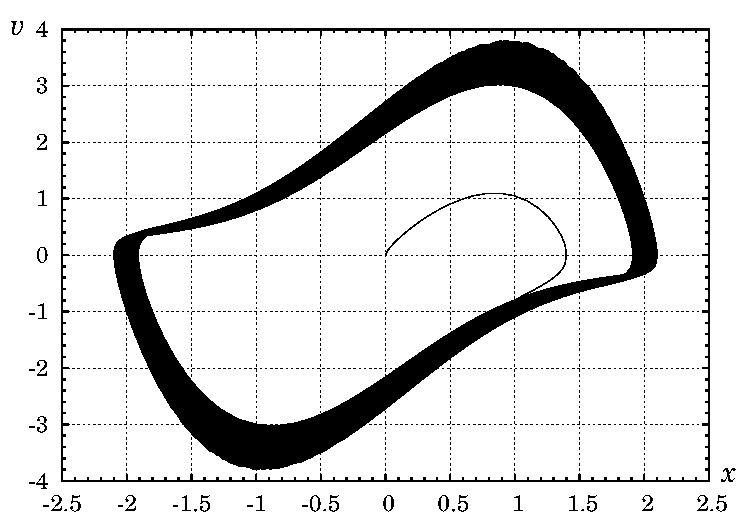
\includegraphics[width=0.5\textwidth]{p/cha/vdp_phase.pdf} }
\caption{Фазовый портрет системы Ван-дер-Поля (\ref{atu:eq:vdp})}
\label{atu:f:vdp_phase}
\end{figure}

% }}}2


\subsection{Анализ и выбор критериев}  % {{{2

Критерий:
$\overline{T}$ + люфт + sign.

Альтернативный критерий:
$\overline{x^2}$

% }}}2

\subsection{Тестовая задача идентификации для системы Ван-дер-Поля}  % {{{2

% }}}2


\subsection{Влияние параметров системы идентификации на ошибку идентификации для системы Ван-дер-Поля}  % {{{2


Зависимости здесь

% }}}2

\subsection{Выводы}  % {{{2

Выводы

% }}}2



% }}}1

% vim: fdm=marker foldlevelstart=3 fdc=4 ft=tex
